\chapter{Known vulnerabilities}
\label{kv}
There are several known security vulnerabilities with the current design.
As said in section \ref{pb-aim} an incremental approach was taken.
As such, the design is part of a bigger system that as a whole is to be deployed in the real world.
In this section we will describe the known vulnerabilities
and explain the future work that is needed to solve these.

\section{Branch attack}
In this section we will explain an attack that can be done by a malicious node M.
The attack consists of obscuring a part of his transaction history.
M creates a new branch of his transaction history that is more favourable to him.

\subsection{Abandoning full transaction history distribution}
One of the main pillars of the design is to not distribute
and have one common, full transaction history between every peer.
While this is the main pillar of design for the blockchain of Bitcoins.
The reasoning behind the idea to abandon is that a common, full truth
will limit the amount of interactions that can be processed
or the participiation of less powerfull machines.

The reason for the limitation is that every interactions will have to be distributed to every peer in the network.
Every transaction has to be processed by every node at the cost of bandwidth, compute power and storage.
The cost might be very limited for a single transaction,
but with greater scale these cost will add up.
The amount of these three resources is limited and will limit the amount of transactions that can be processed.

The limitation can be delayed by naturally excluding participation of less powerfull devices.
For example, mobile devices have generally much less storage available.
When the full transaction history becomes too large,
participation of these mobile devices is excluded due to the fact that they cannot fully store the transaction history.
This problem can be seen to affect Bitcoins and has been demonstrated in section \ref{bitcoin-limit-size}.

\subsection{Alternating partial transaction history}
A malicious node M has his own chain of transactions
and he wants to falsify his transactions after a certain point.
He wants to rewrite his transaction history from that point and create an alternate transaction history.
M wants to do this to whitewash his reputation.
The node can simply choose to forget and obscure blocks after that point.
A new branch will be created by chaining new blocks to the desired point in history.

\begin{figure}
	\centerline{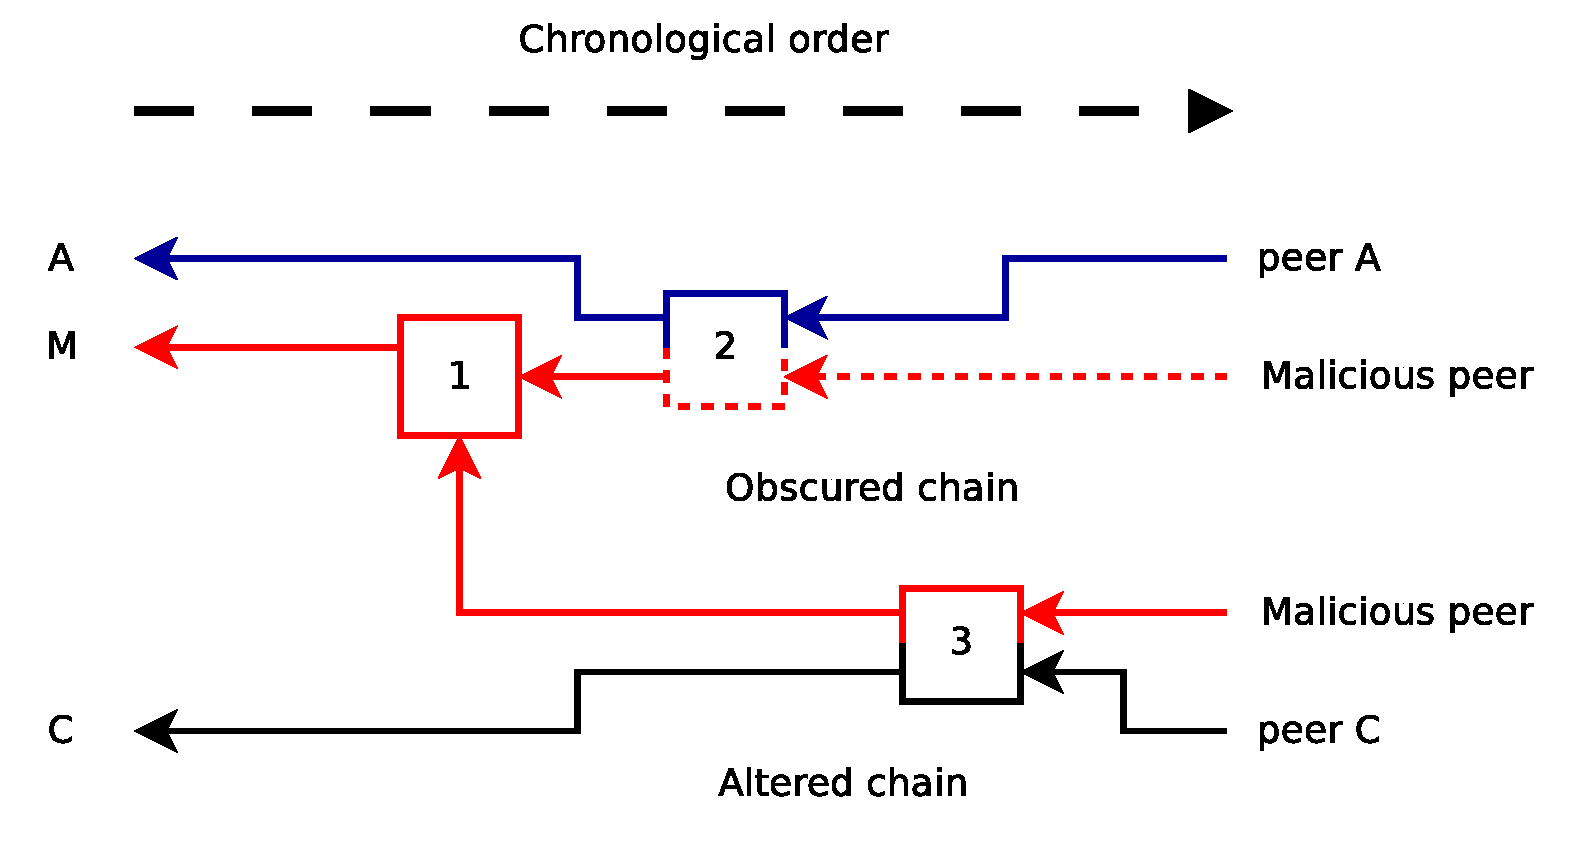
\includegraphics[scale=0.3]{problems/figs/branch.eps}}
	\caption{Example of a branch created by M.}
	\label{fig:problem-branch-obscure}
\end{figure}

In Figure \ref{fig:problem-branch-obscure} an example can be seen of a branch created by M.
In this example M tries to obscure block 2 and any subsequent blocks from C.
When C requests the transaction history of M, M will only send the transaction history up to block 1.
When M and C create a block together,
M will reuse the hash of block 1 in the new block.
For clarity of the diagram, the node interacting with M in block 1 is not displayed.

Now malicious node M does have the problem that not only he knows his transaction history.
When M interacted with node A a block was created that M tries to obscure.
A has this block in his own chain
and therefore knows about it being part of the transaction history of M.
This can be seen in the example in Figure \ref{fig:problem-branch-obscure}.

M will want to reduce the likelyhood of the detection of his fraud.
If his fraud is detected, he might be punished and no longer to continue his abuse.
The first way to minimize detection is to choose
to only interact with new nodes that do not know about the alternate part of the transaction history.
Nodes that have requested an alternate part of the transaction history
or that have been interacted directly with are no longer interacted with.
In a sufficiently healthy network this will result in node M being able to find new nodes to help him.

\begin{figure}
	\centerline{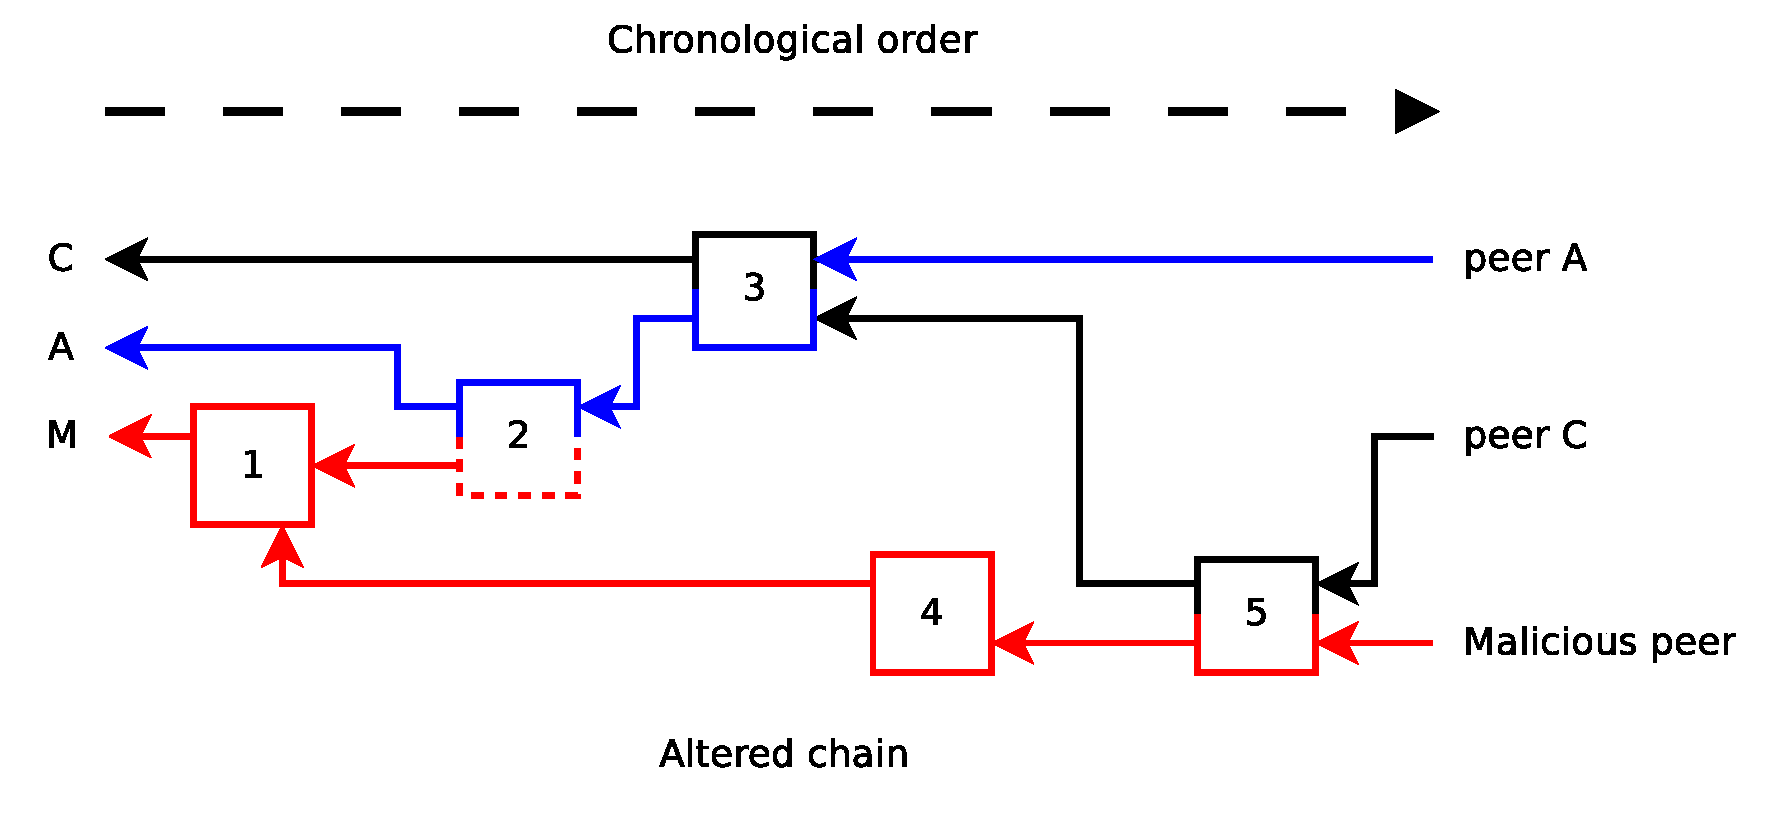
\includegraphics[scale=0.3]{problems/figs/branch-fraud-detected.eps}}
	\caption{Detectable fraud by C.}
	\label{fig:problem-branch-preknowledge}
\end{figure}

There is another example that will expose the fraud of M.
This example can be seen in Figure \ref{fig:problem-branch-preknowledge}.
A node C might still exposes the cheating of M by chance.
C can have an interaction with node A by coincidence.
Before creating block 3 C will request the transaction history of node A containing an obscured block of M.
Now when M wants to interact with C, M will want to create block 5.
When C requests the full transaction history of M, it will detect that the transaction history of M no longer contains block 2.
This exposes the fraud of M.

But C will have no sure way of exposing this type of fraud by his own doing,
except for requesting every transaction history of every node in the system.
This is in a way a common, full transaction history and was chosen to be avoided by the design to become more scalable.
C can limited the possibility of the attack by increasing his knowledge by collecting more transaction history of other nodes.
If node A or B stop participating and exit the network,
then C will have no way of detecting the fraud by M.

The second way M can limit the exposure of his cheating is in a more sophisticated way.
He can present several, different transaction history to different nodes.
M will continue keeping track of the unmodified transaction history.
When M wants to interact with A or B, both knowing this transaction history, he will present this transaction history.
So M can still interact with A and B.
But when interacting with C he will present his alternate transaction history.
C will only expose the fraud in the same way as previously.

\subsection{Possibility of attack and likelyhood of detecting fraud}
This attack can always be done M and is not limited to circumstances.
Also the attack is not limited and M can try to fool any number of other nodes C.
As shown in Figure \ref{fig:branch-multiple}.

\begin{figure}
	\centerline{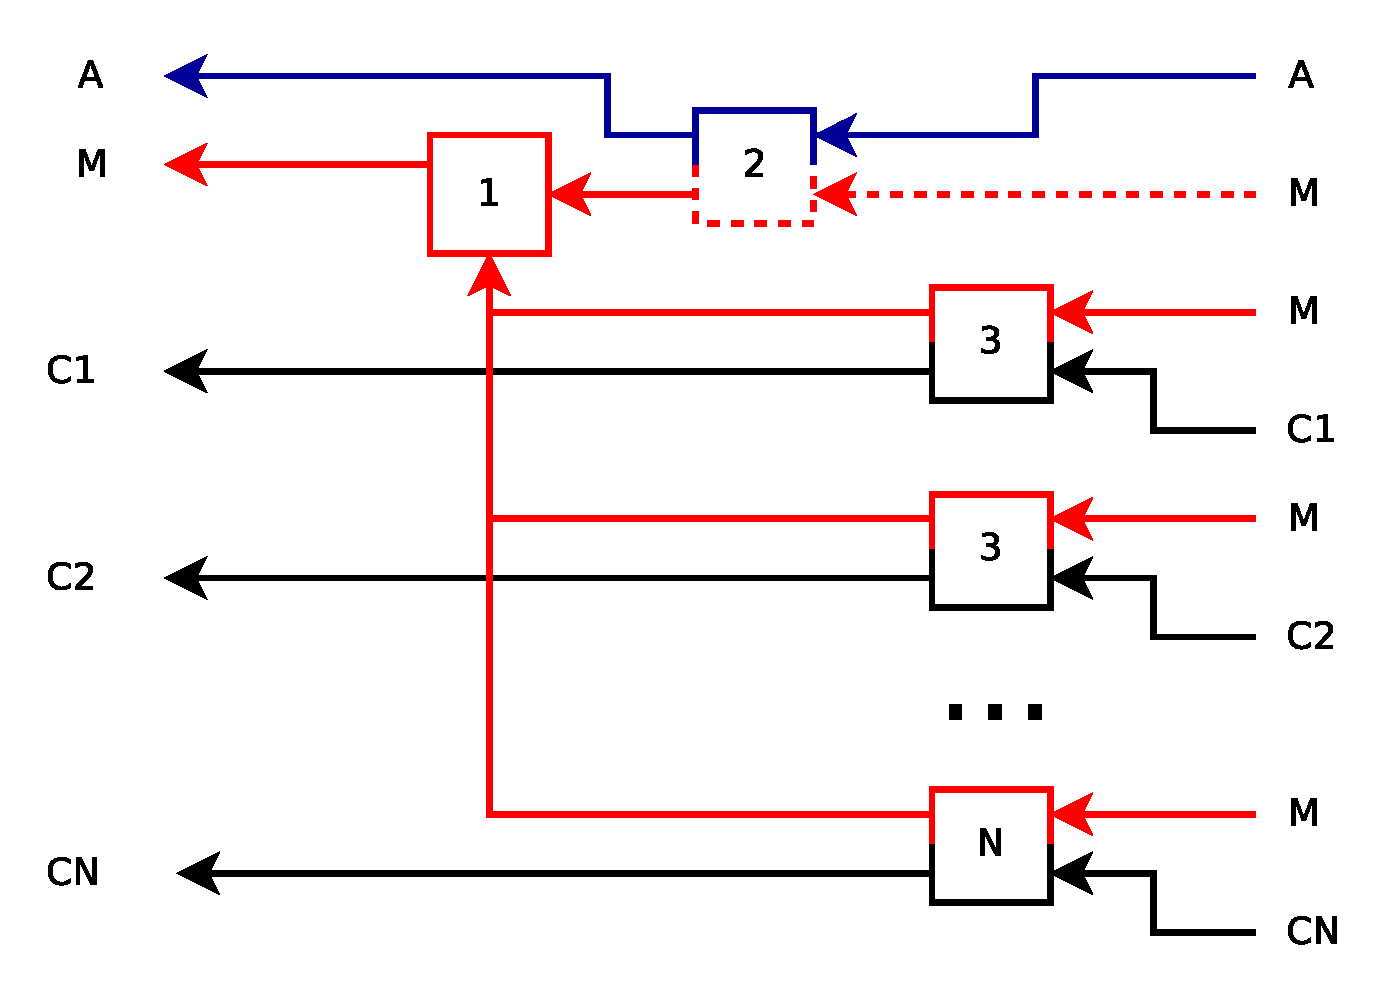
\includegraphics[scale=0.3]{problems/figs/branch-multiple.eps}}
	\caption{Example of multiple branches created by M.}
	\label{fig:branch-multiple}
\end{figure}



The likelyhood of exposing this attack depends on several factors
and will be the only factor to limit M in performing this fraud.
The likelihood depends on:
\begin{itemize}
\item Size of the network
\item Likelihood of interactions between A or B and C
\end{itemize}

All these properties will influence the chance of C coming across an obscured block.

\subsection{Possible punishment of this attack}
When the fraud is detected C can only punish M by no longer interacting with him.
There is currently no way of making it globally know to every node in the network that fraud was committed.
So only M is punished by C and can continue his abuse of other nodes in the network.
It is recommended as future work to do so.

\section{The Sybil Attack}

In this section we will explain the Sybil Attack\cite{douceur-sybil}
and how it can be used in the MultiChain system to create an artificial reputation.
An universallly applicable solution has not yet be found\cite{levine-sybilsurvey}.

\subsection{Using fake indentities}
In large distributed systems convincingly distinct identities can be presented
that are infact all under the control of a single adversary M.
Identities can be public keys like in the Dispersy system
or other abstractions of information without direct physical knowledge.
These identities can participate in the system acting like normal agents,
but they can also help each other malificiently to boost each other towards a common goal.

In the MultiChain system the attack is done in the following way.
M creates several other identities besides his own.
This involves generating several key pairs.
Now M controls several identities that can be presented convincingly.
The key pairs do not have to be linked to a node responding to requests.
Failure of nodes are typical in large distributed systems.

Using these key pairs M can now generate an artificial reputation.
Transactions between M and the fake identities are generated by M.
These are signed using the keys of the fake identities.
Using a single transaction it cannot be determined if it is between two distinct identities or a single distinct identity and a fake identity.

\begin{figure}
	\centerline{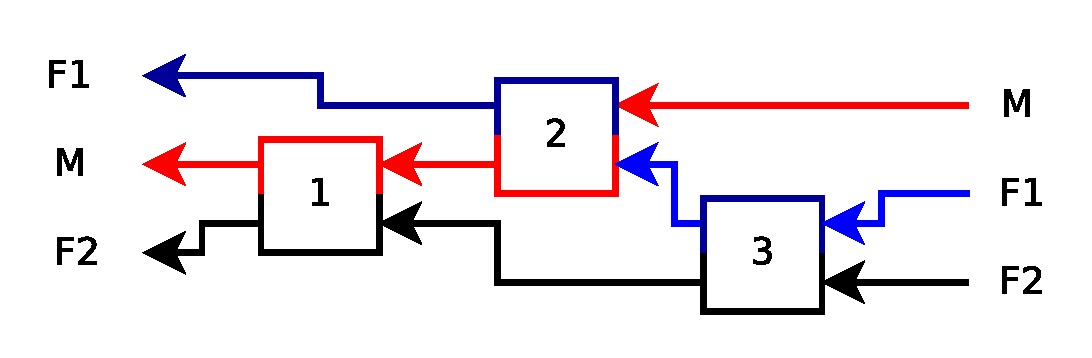
\includegraphics[scale=0.3]{problems/figs/sybil.eps}}
	\caption{The sybil attack by M.}
	\label{fig:sybil-example}
\end{figure}

An example of the Sybil Attack can be seen in \ref{fig:sybil-example}.
In this example M is the malificient node and F1 and F2 his fake identities.
Block 1 and block 2 contain a transaction that is favourable to M,
but M has done nothing to deserve these.
Similair blocks like block 3 can be generated between fake identities in an effort to thwart efforts to analyse the network
and detect fake identities.

In this way M is able to boost his reputation without much work.
The more sophisticated the generation is done by M,
the harder it will be to detect that M boosted his reputation using fake identities.
M can then abuse his fake reputation by solliciting cooperation from other nodes in the network.
They will respond positively on the request by M based upon the false reputation M claims to have.

\subsection{Validating Identities}
A node can have three potential sources of validation of distinct identities:
\begin{itemize}
\item Itself
\item Other entitites
\item A trusted, central authority
\end{itemize}

A node itself could try to directly validate two identities to be distinct.
It would challenge several identities to complete a task that only two entities could complete.
The task would require more resources then a single entity possesses and will be issued simultaneously to all identities.
If the identities complete the task, they have proven to be distinct.
Example of required resources are communication, storage and computation.
These challenges can scale to validate more entities at once.

Indirect validation can be used by a node to by delegating validation to other entities.
A node could accept additional identities to be distinct when an accepted identity vouches for it.
The node has the delegated responsibility to challenge the entity with a challenge.
This would limit the total amount of challenges needed.
But an obvious pitfall of delegating this to other identities is that these can vouch for fraudelent identities.
Next to this, it involves an increase in complexity as the challenges still have to be issued concurrently.

But these challenges are highly indesirable.
These challenges require by definition to occupy between two nodes a limited resource to the maximum capacity of a single node.
While not providing any additional functionality beyond asserting distinct identities.
These challenges also prove inworkable when entities have hugely different amount of resources available.
No challenge can be constructed that can be worked by less powerfull devices,
that could not be worked several times by more powerfull devices.

Next to this, these challenges are only usable with nodes that are active and responding to challenges.
If a node becomes inactive it cannot be ascertained if the node is a fake identity.
But this identity still makes claim about a reputation of another entity.
A choice has to be made between either not counting these claims and allow for a drop in reputation of a node or
allow claims that cannot be validated to be taken into account.
Both options lower the usability of the system.

A trusted, central authority would be able to vouch for distinct indentities
if it has an other way outside the system of asserting that it indeed is a distinct identity.
Approaches exists that implicitly rely on the authority of a trusted agency.
But a central authority goes against the principles of a peer-to-peer network.

Several other defenses against the Sybil Attack have been proposed\cite{newsome-sybil}\cite{dinger-sybil}
or variants on the defenses stated here\cite{levine-sybilsurvey}.
But these either have the same limitation and are minor improvements or are non-applicable for MultiChain.

\subsection{Possibility of attack and likelyhood of detecting fraud}
For M to conduct the Sybil Attack he will need to generate a set of key pairs.
This is trivial to do and Dispersy provides functionality to do this very easily.

%TODO Timing of generating several keys

With these keys M has to generate blocks.

%TODO timing of generating blocks

Sybil Attack can have a wide range of sophistication.
Ranging from a large amount of fake identities with a large amount of transaction between them
to a single, fake identity boosting the reputation of M in a couple of transaction.
Even these simple Sybil Attack are hard to defend against if these are not done to obviously.



